
%% bare_conf.tex
%% V1.3
%% 2007/01/11
%% by Michael Shell
%% See:
%% http://www.michaelshell.org/
%% for current contact information.
%%
%% This is a skeleton file demonstrating the use of IEEEtran.cls
%% (requires IEEEtran.cls version 1.7 or later) with an IEEE conference paper.
%%
%% Support sites:
%% http://www.michaelshell.org/tex/ieeetran/
%% http://www.ctan.org/tex-archive/macros/latex/contrib/IEEEtran/
%% and
%% http://www.ieee.org/

%%*************************************************************************
%% Legal Notice:
%% This code is offered as-is without any warranty either expressed or
%% implied; without even the implied warranty of MERCHANTABILITY or
%% FITNESS FOR A PARTICULAR PURPOSE! 
%% User assumes all risk.
%% In no event shall IEEE or any contributor to this code be liable for
%% any damages or losses, including, but not limited to, incidental,
%% consequential, or any other damages, resulting from the use or misuse
%% of any information contained here.
%%
%% All comments are the opinions of their respective authors and are not
%% necessarily endorsed by the IEEE.
%%
%% This work is distributed under the LaTeX Project Public License (LPPL)
%% ( http://www.latex-project.org/ ) version 1.3, and may be freely used,
%% distributed and modified. A copy of the LPPL, version 1.3, is included
%% in the base LaTeX documentation of all distributions of LaTeX released
%% 2003/12/01 or later.
%% Retain all contribution notices and credits.
%% ** Modified files should be clearly indicated as such, including  **
%% ** renaming them and changing author support contact information. **
%%
%% File list of work: IEEEtran.cls, IEEEtran_HOWTO.pdf, bare_adv.tex,
%%                    bare_conf.tex, bare_jrnl.tex, bare_jrnl_compsoc.tex
%%*************************************************************************

% *** Authors should verify (and, if needed, correct) their LaTeX system  ***
% *** with the testflow diagnostic prior to trusting their LaTeX platform ***
% *** with production work. IEEE's font choices can trigger bugs that do  ***
% *** not appear when using other class files.                            ***
% The testflow support page is at:
% http://www.michaelshell.org/tex/testflow/



% Note that the a4paper option is mainly intended so that authors in
% countries using A4 can easily print to A4 and see how their papers will
% look in print - the typesetting of the document will not typically be
% affected with changes in paper size (but the bottom and side margins will).
% Use the testflow package mentioned above to verify correct handling of
% both paper sizes by the user's LaTeX system.
%
% Also note that the "draftcls" or "draftclsnofoot", not "draft", option
% should be used if it is desired that the figures are to be displayed in
% draft mode.
%
%\documentclass[10pt, conference, compsocconf]{IEEEtran}
\documentclass[conference]{IEEEtran}
% Add the compsocconf option for Computer Society conferences.
%
% If IEEEtran.cls has not been installed into the LaTeX system files,
% manually specify the path to it like:
% \documentclass[conference]{../sty/IEEEtran}

\usepackage{booktabs} % For formal tables
\usepackage{minted}
\usepackage{graphicx}
\usepackage{arydshln}
\usepackage{subcaption}
\usepackage{times}
\usepackage{hyperref}
\usepackage[normalem]{ulem}
%\hypersetup{
%    colorlinks=true,
%    linkcolor=blue,
%    filecolor=magenta,      
%    urlcolor=cyan,
%}
%\usepackage[noadjust]{cite}
\let\OLDthebibliography\thebibliography
\renewcommand\thebibliography[1]{
  \OLDthebibliography{#1}
  \setlength{\parskip}{0pt}
  \setlength{\itemsep}{0pt plus 0.3ex}
}
\setlength{\belowcaptionskip}{-5pt}
\usepackage{caption}

%%%%%%%%%%%%%%%%%%%%%%%%%%%%%%%%%%%%%%%%%%%%%%%%%%
% Uncomment for diff 
%\newcommand{\newcomment}[1]{{\textcolor{blue}{#1}}}
%\newcommand{\oldcomment}[1]{{\textcolor{red}{\textbf{\sout{#1}}}}}
%\newcommand{\addressesissue}[1]{{\textcolor{red}{{\it (Addresses issue(s): {#1})}}}}

% Uncomment for camera-ready
\newcommand{\newcomment}[1]{{\textcolor{black}{#1}}}
\newcommand{\oldcomment}[1]{}
\newcommand{\addressesissue}[1]{}
%%%%%%%%%%%%%%%%%%%%%%%%%%%%%%%%%%%%%%%%%%%%%%%%%%

%% Copyright
%%\setcopyright{none}
%%\setcopyright{acmcopyright}
%%\setcopyright{acmlicensed}
%\setcopyright{rightsretained}
%%\setcopyright{usgov}
%%\setcopyright{usgovmixed}
%%\setcopyright{cagov}
%%\setcopyright{cagovmixed}
%
%
%% DOI
%\acmDOI{10.475/123_4}
%
%% ISBN
%\acmISBN{123-4567-24-567/08/06}
%
%%Conference
%\acmConference[WOODSTOCK'97]{ACM Woodstock conference}{July 1997}{El
%  Paso, Texas USA} 
%\acmYear{1997}
%\copyrightyear{2016}
%
%\acmPrice{15.00}





% Some very useful LaTeX packages include:
% (uncomment the ones you want to load)


% *** MISC UTILITY PACKAGES ***
%
%\usepackage{ifpdf}
% Heiko Oberdiek's ifpdf.sty is very useful if you need conditional
% compilation based on whether the output is pdf or dvi.
% usage:
% \ifpdf
%   % pdf code
% \else
%   % dvi code
% \fi
% The latest version of ifpdf.sty can be obtained from:
% http://www.ctan.org/tex-archive/macros/latex/contrib/oberdiek/
% Also, note that IEEEtran.cls V1.7 and later provides a builtin
% \ifCLASSINFOpdf conditional that works the same way.
% When switching from latex to pdflatex and vice-versa, the compiler may
% have to be run twice to clear warning/error messages.






% *** CITATION PACKAGES ***
%
%\usepackage{cite}
% cite.sty was written by Donald Arseneau
% V1.6 and later of IEEEtran pre-defines the format of the cite.sty package
% \cite{} output to follow that of IEEE. Loading the cite package will
% result in citation numbers being automatically sorted and properly
% "compressed/ranged". e.g., [1], [9], [2], [7], [5], [6] without using
% cite.sty will become [1], [2], [5]--[7], [9] using cite.sty. cite.sty's
% \cite will automatically add leading space, if needed. Use cite.sty's
% noadjust option (cite.sty V3.8 and later) if you want to turn this off.
% cite.sty is already installed on most LaTeX systems. Be sure and use
% version 4.0 (2003-05-27) and later if using hyperref.sty. cite.sty does
% not currently provide for hyperlinked citations.
% The latest version can be obtained at:
% http://www.ctan.org/tex-archive/macros/latex/contrib/cite/
% The documentation is contained in the cite.sty file itself.






% *** GRAPHICS RELATED PACKAGES ***
%
\ifCLASSINFOpdf
  % \usepackage[pdftex]{graphicx}
  % declare the path(s) where your graphic files are
  % \graphicspath{{../pdf/}{../jpeg/}}
  % and their extensions so you won't have to specify these with
  % every instance of \includegraphics
  % \DeclareGraphicsExtensions{.pdf,.jpeg,.png}
\else
  % or other class option (dvipsone, dvipdf, if not using dvips). graphicx
  % will default to the driver specified in the system graphics.cfg if no
  % driver is specified.
  % \usepackage[dvips]{graphicx}
  % declare the path(s) where your graphic files are
  % \graphicspath{{../eps/}}
  % and their extensions so you won't have to specify these with
  % every instance of \includegraphics
  % \DeclareGraphicsExtensions{.eps}
\fi
% graphicx was written by David Carlisle and Sebastian Rahtz. It is
% required if you want graphics, photos, etc. graphicx.sty is already
% installed on most LaTeX systems. The latest version and documentation can
% be obtained at: 
% http://www.ctan.org/tex-archive/macros/latex/required/graphics/
% Another good source of documentation is "Using Imported Graphics in
% LaTeX2e" by Keith Reckdahl which can be found as epslatex.ps or
% epslatex.pdf at: http://www.ctan.org/tex-archive/info/
%
% latex, and pdflatex in dvi mode, support graphics in encapsulated
% postscript (.eps) format. pdflatex in pdf mode supports graphics
% in .pdf, .jpeg, .png and .mps (metapost) formats. Users should ensure
% that all non-photo figures use a vector format (.eps, .pdf, .mps) and
% not a bitmapped formats (.jpeg, .png). IEEE frowns on bitmapped formats
% which can result in "jaggedy"/blurry rendering of lines and letters as
% well as large increases in file sizes.
%
% You can find documentation about the pdfTeX application at:
% http://www.tug.org/applications/pdftex





% *** MATH PACKAGES ***
%
%\usepackage[cmex10]{amsmath}
% A popular package from the American Mathematical Society that provides
% many useful and powerful commands for dealing with mathematics. If using
% it, be sure to load this package with the cmex10 option to ensure that
% only type 1 fonts will utilized at all point sizes. Without this option,
% it is possible that some math symbols, particularly those within
% footnotes, will be rendered in bitmap form which will result in a
% document that can not be IEEE Xplore compliant!
%
% Also, note that the amsmath package sets \interdisplaylinepenalty to 10000
% thus preventing page breaks from occurring within multiline equations. Use:
%\interdisplaylinepenalty=2500
% after loading amsmath to restore such page breaks as IEEEtran.cls normally
% does. amsmath.sty is already installed on most LaTeX systems. The latest
% version and documentation can be obtained at:
% http://www.ctan.org/tex-archive/macros/latex/required/amslatex/math/





% *** SPECIALIZED LIST PACKAGES ***
%
%\usepackage{algorithmic}
% algorithmic.sty was written by Peter Williams and Rogerio Brito.
% This package provides an algorithmic environment fo describing algorithms.
% You can use the algorithmic environment in-text or within a figure
% environment to provide for a floating algorithm. Do NOT use the algorithm
% floating environment provided by algorithm.sty (by the same authors) or
% algorithm2e.sty (by Christophe Fiorio) as IEEE does not use dedicated
% algorithm float types and packages that provide these will not provide
% correct IEEE style captions. The latest version and documentation of
% algorithmic.sty can be obtained at:
% http://www.ctan.org/tex-archive/macros/latex/contrib/algorithms/
% There is also a support site at:
% http://algorithms.berlios.de/index.html
% Also of interest may be the (relatively newer and more customizable)
% algorithmicx.sty package by Szasz Janos:
% http://www.ctan.org/tex-archive/macros/latex/contrib/algorithmicx/




% *** ALIGNMENT PACKAGES ***
%
%\usepackage{array}
% Frank Mittelbach's and David Carlisle's array.sty patches and improves
% the standard LaTeX2e array and tabular environments to provide better
% appearance and additional user controls. As the default LaTeX2e table
% generation code is lacking to the point of almost being broken with
% respect to the quality of the end results, all users are strongly
% advised to use an enhanced (at the very least that provided by array.sty)
% set of table tools. array.sty is already installed on most systems. The
% latest version and documentation can be obtained at:
% http://www.ctan.org/tex-archive/macros/latex/required/tools/


%\usepackage{mdwmath}
%\usepackage{mdwtab}
% Also highly recommended is Mark Wooding's extremely powerful MDW tools,
% especially mdwmath.sty and mdwtab.sty which are used to format equations
% and tables, respectively. The MDWtools set is already installed on most
% LaTeX systems. The lastest version and documentation is available at:
% http://www.ctan.org/tex-archive/macros/latex/contrib/mdwtools/


% IEEEtran contains the IEEEeqnarray family of commands that can be used to
% generate multiline equations as well as matrices, tables, etc., of high
% quality.


%\usepackage{eqparbox}
% Also of notable interest is Scott Pakin's eqparbox package for creating
% (automatically sized) equal width boxes - aka "natural width parboxes".
% Available at:
% http://www.ctan.org/tex-archive/macros/latex/contrib/eqparbox/





% *** SUBFIGURE PACKAGES ***
%\usepackage[tight,footnotesize]{subfigure}
% subfigure.sty was written by Steven Douglas Cochran. This package makes it
% easy to put subfigures in your figures. e.g., "Figure 1a and 1b". For IEEE
% work, it is a good idea to load it with the tight package option to reduce
% the amount of white space around the subfigures. subfigure.sty is already
% installed on most LaTeX systems. The latest version and documentation can
% be obtained at:
% http://www.ctan.org/tex-archive/obsolete/macros/latex/contrib/subfigure/
% subfigure.sty has been superceeded by subfig.sty.



%\usepackage[caption=false]{caption}
%\usepackage[font=footnotesize]{subfig}
% subfig.sty, also written by Steven Douglas Cochran, is the modern
% replacement for subfigure.sty. However, subfig.sty requires and
% automatically loads Axel Sommerfeldt's caption.sty which will override
% IEEEtran.cls handling of captions and this will result in nonIEEE style
% figure/table captions. To prevent this problem, be sure and preload
% caption.sty with its "caption=false" package option. This is will preserve
% IEEEtran.cls handing of captions. Version 1.3 (2005/06/28) and later 
% (recommended due to many improvements over 1.2) of subfig.sty supports
% the caption=false option directly:
%\usepackage[caption=false,font=footnotesize]{subfig}
%
% The latest version and documentation can be obtained at:
% http://www.ctan.org/tex-archive/macros/latex/contrib/subfig/
% The latest version and documentation of caption.sty can be obtained at:
% http://www.ctan.org/tex-archive/macros/latex/contrib/caption/




% *** FLOAT PACKAGES ***
%
%\usepackage{fixltx2e}
% fixltx2e, the successor to the earlier fix2col.sty, was written by
% Frank Mittelbach and David Carlisle. This package corrects a few problems
% in the LaTeX2e kernel, the most notable of which is that in current
% LaTeX2e releases, the ordering of single and double column floats is not
% guaranteed to be preserved. Thus, an unpatched LaTeX2e can allow a
% single column figure to be placed prior to an earlier double column
% figure. The latest version and documentation can be found at:
% http://www.ctan.org/tex-archive/macros/latex/base/



%\usepackage{stfloats}
% stfloats.sty was written by Sigitas Tolusis. This package gives LaTeX2e
% the ability to do double column floats at the bottom of the page as well
% as the top. (e.g., "\begin{figure*}[!b]" is not normally possible in
% LaTeX2e). It also provides a command:
%\fnbelowfloat
% to enable the placement of footnotes below bottom floats (the standard
% LaTeX2e kernel puts them above bottom floats). This is an invasive package
% which rewrites many portions of the LaTeX2e float routines. It may not work
% with other packages that modify the LaTeX2e float routines. The latest
% version and documentation can be obtained at:
% http://www.ctan.org/tex-archive/macros/latex/contrib/sttools/
% Documentation is contained in the stfloats.sty comments as well as in the
% presfull.pdf file. Do not use the stfloats baselinefloat ability as IEEE
% does not allow \baselineskip to stretch. Authors submitting work to the
% IEEE should note that IEEE rarely uses double column equations and
% that authors should try to avoid such use. Do not be tempted to use the
% cuted.sty or midfloat.sty packages (also by Sigitas Tolusis) as IEEE does
% not format its papers in such ways.





% *** PDF, URL AND HYPERLINK PACKAGES ***
%
%\usepackage{url}
% url.sty was written by Donald Arseneau. It provides better support for
% handling and breaking URLs. url.sty is already installed on most LaTeX
% systems. The latest version can be obtained at:
% http://www.ctan.org/tex-archive/macros/latex/contrib/misc/
% Read the url.sty source comments for usage information. Basically,
% \url{my_url_here}.





% *** Do not adjust lengths that control margins, column widths, etc. ***
% *** Do not use packages that alter fonts (such as pslatex).         ***
% There should be no need to do such things with IEEEtran.cls V1.6 and later.
% (Unless specifically asked to do so by the journal or conference you plan
% to submit to, of course. )


% correct bad hyphenation here
\hyphenation{op-tical net-works semi-conduc-tor}


\begin{document}
%
% paper title
% can use linebreaks \\ within to get better formatting as desired
%\title{Bare Demo of IEEEtran.cls for IEEECS Conferences}
\title{Cudele: An API and Framework for Programmable\\Consistency and Durability in a Global Namespace}


% author names and affiliations
% use a multiple column layout for up to two different
% affiliations

%\author{\IEEEauthorblockN{Authors Name/s per 1st Affiliation (Author)}
%\IEEEauthorblockA{line 1 (of Affiliation): dept. name of organization\\
%line 2: name of organization, acronyms acceptable\\
%line 3: City, Country\\
%line 4: Email: name@xyz.com}
%\and
%\IEEEauthorblockN{Authors Name/s per 2nd Affiliation (Author)}
%\IEEEauthorblockA{line 1 (of Affiliation): dept. name of organization\\
%line 2: name of organization, acronyms acceptable\\
%line 3: City, Country\\
%line 4: Email: name@xyz.com}
%}

\author{
\IEEEauthorblockN{Michael A. Sevilla, Ivo Jimenez, Noah Watkins, Jeff LeFevre,}
\IEEEauthorblockN{Peter Alvaro, Shel Finkelstein, Patrick Donnelly*, Carlos Maltzahn}
\IEEEauthorblockN{University of California, Santa Cruz; *Red Hat, Inc.}
\IEEEauthorblockA{\{msevilla, ivo, jayhawk, jlefevre\}@soe.ucsc.edu, \{palvaro, shel, carlosm\}@ucsc.edu, pdonnell@redhat.com}}

% conference papers do not typically use \thanks and this command
% is locked out in conference mode. If really needed, such as for
% the acknowledgment of grants, issue a \IEEEoverridecommandlockouts
% after \documentclass

% for over three affiliations, or if they all won't fit within the width
% of the page, use this alternative format:
% 
%\author{\IEEEauthorblockN{Michael Shell\IEEEauthorrefmark{1},
%Homer Simpson\IEEEauthorrefmark{2},
%James Kirk\IEEEauthorrefmark{3}, 
%Montgomery Scott\IEEEauthorrefmark{3} and
%Eldon Tyrell\IEEEauthorrefmark{4}}
%\IEEEauthorblockA{\IEEEauthorrefmark{1}School of Electrical and Computer Engineering\\
%Georgia Institute of Technology,
%Atlanta, Georgia 30332--0250\\ Email: see http://www.michaelshell.org/contact.html}
%\IEEEauthorblockA{\IEEEauthorrefmark{2}Twentieth Century Fox, Springfield, USA\\
%Email: homer@thesimpsons.com}
%\IEEEauthorblockA{\IEEEauthorrefmark{3}Starfleet Academy, San Francisco, California 96678-2391\\
%Telephone: (800) 555--1212, Fax: (888) 555--1212}
%\IEEEauthorblockA{\IEEEauthorrefmark{4}Tyrell Inc., 123 Replicant Street, Los Angeles, California 90210--4321}}




% use for special paper notices
%\IEEEspecialpapernotice{(Invited Paper)}




% make the title area
\maketitle


\input{sections/0_abstract}
\begin{IEEEkeywords}
file systems; high performance computing; data storage systems; system software

\end{IEEEkeywords}


% For peer review papers, you can put extra information on the cover
% page as needed:
% \ifCLASSOPTIONpeerreview
% \begin{center} \bfseries EDICS Category: 3-BBND \end{center}
% \fi
%
% For peerreview papers, this IEEEtran command inserts a page break and
% creates the second title. It will be ignored for other modes.
\IEEEpeerreviewmaketitle


\section{Introduction}

% What is the problem?
File system metadata services in HPC and large-scale data centers have
scalability problems because common tasks, like
checkpointing~\cite{bent_plfs_2009} or scanning the file
system~\cite{zheng:pdsw2014-batchfs}, contend for the same directories and
inodes. Applications perform better with dedicated metadata
servers~\cite{sevilla:sc15-mantle, ren:sc2014-indexfs} but provisioning a
metadata server for every \newcomment{client}\footnote{In this paper, ``client"
is a storage client or application that interacts with the metadata server,
``administrator" is a system administrator that configures the storage, and
``end-users" interact with the file system via home directories or runtimes.  }
is unreasonable. This problem is exacerbated by current hardware and software
trends; for example,  HPC architectures are transitioning from complex storage
stacks with burst buffer, file system, object store, and tape tiers to more
simplified stacks with just a burst buffer and object
store~\cite{bent:login16-hpc-trends}. These types of trends put pressure on
data access because more requests from different nodes end up hitting the same
software layers in parallel and latencies cannot be hidden while data migrates
across tiers.

% What is HPC doing?
To address this, developers are relaxing the consistency and durability
semantics in the file system because weaker guarantees are sufficient for their
applications. For example, many HPC batch jobs do not need the strong
consistency that the file system provides, so
BatchFS~\cite{zheng:pdsw2014-batchfs} and DeltaFS~\cite{zheng:pdsw2015-deltafs}
do more client-side processing and merge updates when the job is done.
Developers in these domains are turning to these non-POSIX IO solutions because
their applications are well-understood ({\it e.g.}, well-defined read/write
phases, synchronization only needed during certain phases, workflows describing
computation, etc.) and because these applications wreak havoc on file systems
designed for general-purpose workloads ({\it e.g.}, checkpoint-restart's N:N
and N:1 create patterns~\cite{bent_plfs_2009}).

\begin{figure}[tb] \centering
\includegraphics[width=0.35\textwidth]{figures/subtree-policies1.png}
\caption{Illustration of subtrees with different semantics co-existing in a
global namespace.  For performance, clients \oldcomment{can} relax consistency/durability on their
subtree ({\it e.g.}, HDFS) or decouple the subtree and move it locally ({\it e.g.}, BatchFS, RAMDisk).\vspace{-3ex}
}\label{fig:subtree-policies} \end{figure}

% One example
One popular approach for relaxing consistency and durability is to ``decouple
the namespace", where clients lock the subtree they want exclusive access to as
a way to tell the file system that the subtree is important or may cause
resource contention in the near-future~\cite{grider:pdsw2015-marfs,
zheng:pdsw2015-deltafs, zheng:pdsw2014-batchfs, ren:sc2014-indexfs,
bent:slides-twotiers}. Then the file system can change its internal structure
to optimize performance. For example, the file system could enter a mode where
clients with decoupled directories perform operations locally and bulk merge their
updates at completion. This delayed merge ({\it i.e.} a form of eventual
consistency) and relaxed durability improves performance and scalability by
avoiding the costs of remote procedure calls (RPCs), synchronization, false
sharing, and serialization.  While the performance benefits of decoupling the
namespace are obvious, applications that rely on the file system's guarantees
must be deployed on an entirely different system or re-written to coordinate
strong consistency/durability themselves. 

% What did we do
%\footnote{HDFS itself is not directly evaluated in this paper, although the
%semantics and their performance is explored in~\S\ref{sec:use-case-1}.} 
To address this problem, we present an API and framework that lets administrators
dynamically control the consistency and durability guarantees for subtrees in
the file system namespace.  Figure~\ref{fig:subtree-policies} shows a potential
setup in our proposed system where a single global namespace has subtrees for
applications optimized with techniques from different state-of-the-art
architectures.  The BatchFS and RAMDisk subtrees are decoupled from the global
namespace and have similar consistency/durability behavior to those systems;
the HDFS subtree has weaker than strong consistency because it lets clients
read files opened for writing~\cite{hakimzadeh:dais14-hdfs-consistency}, which
means that not all updates are immediately seen by all clients; and the POSIX
IO subtree retains the rigidity of POSIX IO's strong consistency.  Subtrees
without policies inherit the consistency/durability semantics of the parent and
future work will examine embeddable or inheritable policies.

Our prototype system, Cudele, achieves this by exposing ``mechanisms" that
\oldcomment{users}\newcomment{administrators} combine to specify their
preferred semantics.  Cudele supports 3 forms of consistency (invisible, weak,
and strong) and 3 degrees of durability (none, local, and global) giving the
\oldcomment{user}\newcomment{administrator} a wide range of policies and
optimizations that can be custom fit to an application. We make the following
contributions:

\begin{enumerate}

  \item A framework/API for assigning consistency/durability policies to
  subtrees in a global namespace; this lets
  \oldcomment{users}\newcomment{administrators} navigate trade-offs of
  different metadata protocols on the same storage system.

  \item

  \oldcomment{This framework lets subtrees with different semantics co-exist in
a global namespace. We show how this} \newcomment{We show that letting
different semantics co-exist in a global namespace scales further and performs
better than systems that use one strategy.}

  \item A prototype that lets \oldcomment{users}\newcomment{administrators}
  custom fit subtrees to applications dynamically. 

\end{enumerate}

\oldcomment{The last contribution lays the groundwork for future work on our
prototype. It is more scalable than the current practice of mounting different
storage systems in a global namespace because there is no need to provision
dedicated storage clusters to applications or move data between these systems.
For example, the results of a Hadoop job do not need to be migrated into a Ceph
file system (CephFS) for other processing; instead the
\oldcomment{users}\newcomment{administrator} can change the semantics of the
HDFS subtree into a CephFS subtree.  This may cause metadata/data movement to
make things strongly consistent again but this is superior to moving all data
across file system boundaries. Our prototype enables studies that adjust these
semantics over {\it time and space}, where subtrees can change their semantics
and migrate around the cluster without ever moving the data they reference.}

% Results
The results in this paper confirm the assertions of ``clean-slate" research of
decoupled namespaces; specifically that these techniques drastically improve
performance.  We go a step further by quantifying the costs of traditional file
system approaches to maintaining consistency (3.37\(\times\) slowdown) and
durability (\(2.4\times\) slowdown).  In our prototype, \newcomment{we also
show the benefits of assigning subtree semantics to certain applications such
as checkpoint-restart (\(91.7\times\) speedup if consistency is fully relaxed),
user home directories (within a 0.03 standard deviation from optimal), and
end-users checking for partial results (only a 2\% overhead).} \oldcomment{we
get an 8\(\times\) speedup and can scale to twice as many clients when we
assign a more relaxed form of consistency and durability to a subtree with a
create-heavy workload.}  We use Ceph as a prototyping platform because it is
used in cloud-based and data center systems and has a presence in
HPC~\cite{wang:pdsw13-ceph-hpc}.

%In the remainder of the paper, Section~\ref{sec:posix-overheads} quantifies the
%cost of POSIX IO consistency and system-defined durability and
%Section~\ref{sec:methodology-decoupled-namespaces} presents the Cudele
%prototype and API. Section~\ref{sec:implementation} describes the Cudele
%mechanisms and shows how re-using internal subsystems results in an
%implementation of less than 500 lines of code. The evaluation in
%Section~\ref{sec:evaluation} quantifies the overheads and performance gains of
%explored and previously unexplored metadata designs.
%Section~\ref{sec:related-work} places Cudele in the context of other related
%work.


\section{POSIX IO Overheads}
\label{sec:posix-overheads}

\begin{figure}[tb] \centering
\includegraphics[width=1\linewidth]{./graphs/overhead-creates.png}
\caption{[\href{https://github.com/michaelsevilla/cudele-popper/blob/master/experiments/baseline-compile/visualize/viz.ipynb}{source}]
For the CephFS metadata server, create-heavy workloads ({\it e.g.},
\texttt{untar}) incur the highest disk, network, and CPU utilization because of
consistency/durability demands.\vspace{-3ex}}\label{fig:overhead-creates}
\end{figure}

In our examination of the overheads of POSIX IO we benchmark and analyze
CephFS, the file system that uses Ceph's object store (RADOS) to
store its data/metadata and a metadata server cluster to service client requests
more quickly.  During this process we discovered, based on the analysis and
breakdown of costs, that durability and consistency have high overhead but we
urge the reader to keep in mind that this file system is an implementation of
one set of design decisions and our goal here is to highlight the effect that
those decisions have on performance.  At the end of each subsection we compare
the approach to ``decoupled namespaces", the technique in related work that
detaches subtrees from the global namespace to relax consistency/durability
guarantees. 

%The RPCs are also serialized because the
%metadata server is single threaded; although na\"{\i}ve, this design is common
%because of the complexity of multi-threaded metadata
%servers~\cite{konstantinos:pdsw2014-lustre-metadata}.  

We use a create-heavy workload for this study because it has high resource
utilization, as shown by the trace of compiling the Linux kernel in a CephFS
mount in Figure~\ref{fig:overhead-creates}.  The \texttt{untar} phase, which is
characterized by many creates, has the highest resource usage (combined CPU,
network, and disk) on the metadata server because of the number of RPCs needed
for consistency and durability.  

\subsection{Durability}
\label{sec:durability}

\begin{figure*}[t]
  \centering
  \begin{subfigure}[b]{.32\linewidth}
      \centering
      \includegraphics[width=1\linewidth]{graphs/slowdown-journal.png}
      \caption{[\href{https://github.com/michaelsevilla/cudele-popper/blob/master/experiments/baseline-durability/visualize/viz.ipynb}{source}]
      effect of journal} \label{fig:overhead-a}
  \end{subfigure}
  \begin{subfigure}[b]{.32\linewidth}
      \centering
      \includegraphics[width=0.98\linewidth]{graphs/slowdown-interfere-scale.png}
      \caption{[\href{https://github.com/michaelsevilla/cudele-popper/blob/master/experiments/baseline-creates/visualize/viz.ipynb}{source}]
      interference hurts variability}
      \label{fig:overhead-b}
  \end{subfigure}
  \begin{subfigure}[b]{.32\linewidth}
      \centering
      \includegraphics[width=1.15\linewidth]{graphs/behavior-interfere.png}
      \caption{[\href{https://github.com/michaelsevilla/cudele-popper/blob/master/experiments/baseline-interfere/visualize/viz.ipynb}{source}]
      interference increases RPCs}
      \label{fig:overhead-c}
  \end{subfigure}
  \caption{\newcomment{The durability and strong consistency slowdown of the
existing CephFS implementation increases as the number of clients scales.
Results in (a) and (b)  are normalized to 1 client that creates 100K files in
isolation.  (a) shows the effect of journaling metadata updates; ``segment(s)"
is the number of journal segments dispatched to disk at once. (b) shows the
slowdown when another client interferes by creating files in all directories
and (c) highlights the cause: }\oldcomment{The overhead of durability and
strong consistency in CephFS. (a) shows the effect of different journal segment
sizes, which are streamed into the object store for fault tolerance. (b) and
(c) show that} when another client interferes, capabilities are revoked and
metadata servers do more work.\vspace{-3ex}} \label{fig:overhead}
\end{figure*}

% what is durability
While durability is not specified by POSIX IO,
\oldcomment{users}\newcomment{administrators} expect that files they create or
modify survive failures.  We define three types of durability: global, local,
and none.  Global durability means that the client or server can fail at any
time and metadata will not be lost because it is ``safe" ({\it i.e.} striped or
replicated across a cluster). Local durability means that metadata can be lost
if the client or server stays down after a failure. None means that metadata is
volatile and that the system provides no guarantees when clients or servers
fail.  None is different than local durability because regardless of the type
of failure, metadata will be lost when components die in a None configuration.

% - sequential IO, trim redundant operations
\textbf{CephFS Design}: A journal of metadata updates that streams into the
resilient object store. Similar to LFS~\cite{rosenblum:acm1992-LFS} 
the metadata journal is designed to be large (on
the order of MBs) which ensures (1) sequential writes into the object store and
(2) the ability for daemons to trim redundant or irrelevant journal entries.
The journal is striped over objects where multiple journal updates can reside
on the same object. There are two tunables\newcomment{, related to groups of
journal events called segments,} for controlling the journal: the segment size
and the dispatch size ({\it i.e.} the number of segments that can be dispatched
at once).  Unless the journal saturates memory or CPU resources, larger values
for these tunables result in better performance.

% purpose of the journal
In addition to the metadata journal, CephFS also represents metadata in RADOS
as a metadata store, where directories and their file inodes are stored as
objects.  The metadata server applies the updates in the journal to the
metadata store when the journal reaches a certain size. The metadata store is
optimized for recovery ({\it i.e.} reading) while the metadata journal is
write-optimized.

%\begin{figure}[tb] \centering
%\includegraphics[width=1\linewidth]{./figures/journal.png} 
%\caption{CephFS has two views of the file system namespace: a journal of
%metadata updates and a metadata store. For fault tolerance, they are stored in
%the object store as segments and fragments, respectively.
%\label{fig:journal}}
%\end{figure}

% Effects on performance
Figure~\ref{fig:overhead-a} shows the effect of journaling with different
\oldcomment{segment sizes; the larger the segment size the bigger that the
writes into the object store are}\newcomment{dispatch sizes, normalized to 1
client that creates 100K files with journaling off (about 654 creates/sec). In
this case a dispatch size of 30 degrades performance the most because the
metadata server is overloaded with requests and cannot spare cycles to manage
concurrent segments.  Tuning and parameter sweeps show that a dispatch size of
10 is the worst and that larger sizes approach a dispatch size of 1; for all
future journal experiments we use a dispatch size of 40 which is a more
realistic configuration.  Although the ``no journal" curve appears flat, it is
actually a slowdown of about \(0.3\times\) per concurrent client; this slowdown
is a result of the peak throughput of a single metadata server, which we found
to be about 3000 operations per second}.  The trade-off for better performance
is memory consumption because a larger
\oldcomment{segment}\newcomment{dispatch} size uses more space for buffering.
\oldcomment{When journaling is on, the metadata server periodically stops serving requests
to flush ({\it i.e.} apply journal updates) to the metadata store.  The journal
overhead is sufficient enough to slow down metadata throughput but not so much
as to overwhelm the bandwidth of the object store.}

\textbf{Comparison to decoupled namespaces}: For BatchFS, if a client fails
when it is writing to the local log-structured merge tree (implemented as an
SSTable~\cite{ren:atc2013-tablefs}) then unwritten metadata operations are
lost. For DeltaFS, if the client fails then, on restart, the computation does
the work again -- since the snapshots of the namespace are never globally
consistent and there is no ground truth.  On the server side, BatchFS and
DeltaFS use IndexFS~\cite{ren:sc2014-indexfs}. IndexFS writes metadata to
SSTables, which initially reside in memory but are later flushed to the
underlying distributed file system.

\subsection{Strong Consistency}
\label{sec:strong-consistency}

Access to metadata in a POSIX IO-compliant file system is strongly consistent, so
reads and writes to the same inode or directory are globally ordered.  The
synchronization and serialization machinery needed to ensure that all clients
see the same state has high overhead.

% inode cache - reduces RPCs (lookups for create, readdirs for stats)

\textbf{CephFS Design}: Capabilities keep metadata strongly consistent. To
reduce the number of RPCs needed for consistency, clients can obtain
capabilities for reading and writing inodes, as well as caching reads,
buffering writes, changing the file size, and performing lazy IO.  To keep
track of the read caching and write buffering capabilities, the clients and
metadata servers agree on the state of each inode using an inode cache.  If a
client has the directory inode cached it can do metadata writes ({\it e.g.},
create) with a single RPC. If the client is not caching the directory inode
then it must do an extra RPC to determine if the file exists.  Unless the
client immediately reads all the inodes in the cache ({\it i.e.} \texttt{ls
-alR}), the inode cache is less useful for create-heavy workloads.

% benefits PROBLEM -- IS THIS THE METADATA PROTOCOL OR JUST THE OVERLOADEDNESS?
\oldcomment{This degradation is shown in Figure~\ref{fig:overhead-b}, where we
scale the number of clients and show the slowdown of the slowest client.  The
results are normalized to a single isolated client without a metadata server
journal and the error bars are the standard deviations of all client runtimes.}
\newcomment{Figure~\ref{fig:overhead-b} shows the slowdown of maintaining
strong consistency when scaling the number of clients.  We plot the slowdown of
the slowest client, normalized to 1 client that creates 100K files (about 513
creates/sec because the journal is turned back on).} For the ``interference"
curve, each client creates files in private directories and at 30 seconds we
launch another process that creates files in those directories. \oldcomment{18
is}\newcomment{20 clients has an asterisk\* because} the maximum number of
clients the metadata server can handle for this metadata-intensive workload
\newcomment{is actually 18}; at higher client load, the metadata server
complains about laggy and unresponsive requests.

\oldcomment{The benefits of caching the directory inode when creating
files}\newcomment{The cause for this slowdown} is shown in
Figure~\ref{fig:overhead-c}. The colors show the behavior of the client for two
different runs.  If only one client is creating files in a directory
(``no interference" curve on \(y1\) axis) then that client can lookup the existence of
new files locally before issuing a create request to the metadata server. If
another client starts creating files in the same directory then the directory
inode transitions out of read caching and the first client must send
\texttt{lookup()}s to the metadata server (``interference" curve on \(y2\) axis).
These extra requests increase the throughput of the ``interference" curve on the
\(y1\) axis because the metadata server can handle the extra load but
performance suffers.  



% TODO: what is the cost of trimming the cache?
% TODO: does CephFS still cache inodes when I turn off caching? Why is still keeping inodes in memory? Gah!

\textbf{Comparison to decoupled namespaces}: Decoupled namespaces
merge batches of metadata operations into the global namespaces when the job
completes.  In BatchFS, the merge is delayed by the application using an API to
switch between asynchronous and synchronous mode. The merge itself is explicitly
managed by the application but future work looks at more automated
methodologies. In DeltaFS, snapshots of the metadata subtrees stays on the client
machines; there is no ground truth and consistent namespaces are constructed
and resolved at application read time or when a 3rd party system ({\it e.g.},
middleware, scheduler, etc.) needs a view of the metadata. As a result, all the
overheads of maintaining consistency that we showed above are delayed until the
merge phase.

\section{Methodology: Global Namespace, Subtree Consistency/Durability}
\label{sec:methodology-decoupled-namespaces}

\begin{figure*}[tb]
  \centering
  \begin{subfigure}[b]{.32\linewidth}
    \centering
    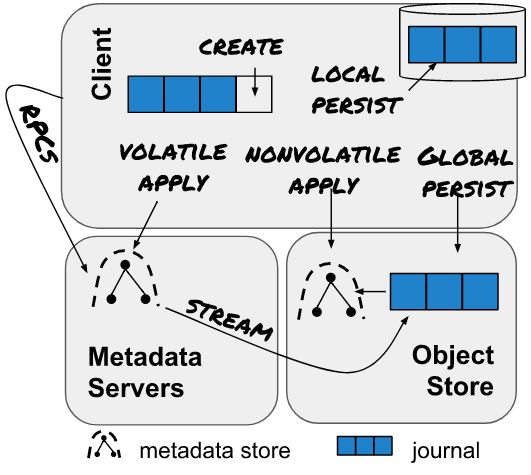
\includegraphics[width=0.7\linewidth]{figures/fig-decouple0.png}
    \caption{Cudele \textbf{mechanisms}
    }\label{fig:decouple}
  \end{subfigure}
  \begin{subfigure}[b]{.32\linewidth}
    \centering
    \scalebox{0.7}{
    \begin{tabular}{ l | l | l | l }
      C \(\rightarrow\) &&& \\
      D \(\downarrow\)  & invisible             & weak                  & strong  \\\hline
      none              & append client journal & append client journal & RPCs    \\
                        &                       & +volatile apply       &         \\
                        &                       &                       &         \\\hdashline
      local             & append client journal & append client journal & RPCs    \\
                        & +local persist        & +local persist        & +local  \\
                        &                       & +volatile apply       & persist \\
                        &                       &                       &         \\\hdashline
      global            & append client journal & append client journal & RPCs    \\
                        & +global persist       & +global persist       & +stream \\
                        &                       & +volatile apply       &         \\
    \end{tabular}}
    \caption{building guarantees from mechanisms
    }\label{table:spectrum}
  \end{subfigure}
  \begin{subfigure}[b]{.32\linewidth}
    \includegraphics[width=1.0\linewidth]{graphs/composable-mechanisms.png}
    \caption{
    [\href{https://github.com/michaelsevilla/cudele-popper/blob/master/experiments/cudele-mechanisms/visualize/viz.ipynb}{source}]
    \textbf{mechanism} performance
    }\label{fig:composable-mechanisms}
  \end{subfigure}
  \caption{Cudele mechanism performance.
    (a) is an illustration of the \textbf{mechanisms} used by applications to build
    semantics. Descriptions are provided by the
    underlined words in Section~\S\ref{sec:the-cudelesfs-mechanisms}.
    (b) shows how users can explore the consistency (C) and
    durability (D) spectrum by composing Cudele mechanisms.
    \newcomment{(c) shows the overhead of processing 100K create events for each mechanism in
    \oldcomment{Table~\ref{table:mechanisms}}\newcomment{Figure~\ref{fig:decouple}},
    normalized to the runtime of writing events to client memory. The far right
    graph shows the cost of building real world systems.}
    \oldcomment{Performance of each mechanism (left) and building the
    consistency/durability semantics of real-world systems (right) for 100K files
    creates from a single client. Results are normalized to the runtime of writing
    events to the client's in-memory journal.}\vspace{-3ex}}
\end{figure*}

%\begin{table}
%\begin{tabular}{ r | l }
%  Mechanism         & Description \\\hline
%  RPCs              & round trip remote procedure calls \\
%  Stream            & stream journal into object store \\
%  Append Client Journal & events appended to in-memory journal \\
%  Volatile Apply & apply to metadata store in memory \\
%  Nonvolatile Apply    & apply to metadata store in obj store \\
%  Local Persist     & journal saved to client's disk \\
%  Global Persist    & journal saved in object store \\
%\end{tabular}
%\caption{Descriptions of the mechanisms. Example compositions are shown in Table~\ref{table:spectrum}.\label{table:mechanisms}} 
%\end{table}

In this section we describe our API and framework that lets
\oldcomment{users}\newcomment{administrators} assign consistency and durability
semantics to subtrees in the global namespace. A \textbf{mechanism} is an
abstraction and basic building block for constructing consistency and
durability guarantees. \oldcomment{Cudele exposes these mechanisms and the
users}\newcomment{The administrator} composes these mechanisms together to
construct \textbf{policies}.  These policies are assigned to subtrees and they
dictate how the file system should handle operations within that subtree.
Below, we describe the mechanisms (which are \underline{underlined}), the
policies, and the API for assigning policies to subtrees.

\subsection{Mechanisms: Building Guarantees}
\label{sec:the-cudelesfs-mechanisms}

% describe the figure
Figure~\ref{fig:decouple} shows the mechanisms (labeled arrows) in Cudele and
which daemon(s) they are performed by. \oldcomment{Table~\ref{table:mechanisms} has a
description of what each mechanism does.}  Decoupled clients use the
\underline{Append Client Journal} mechanism to append metadata updates to a
local, in-memory journal. Clients do not need to check for
consistency when writing events and the metadata server blindly applies the
updates because it assumes the events were already checked for consistency. The
trade-off here is fast performance; it is a dangerous approach but could be
implemented safely if the clients or metadata server are configured to check
the validity of events before writing them.  Once the job is complete, the
system calls mechanisms to achieve the desired consistency/durability
semantics.  Cudele provides a library for clients to link into and all
operations are performed by the client.  

\subsubsection{Mechanisms Used for Consistency} \underline{RPCs} send remote
procedure calls for every metadata operation from the client to the metadata
server, assuming the request cannot be satisfied by the inode cache. This
mechanism is part of the default CephFS implementation and is the strongest
form of consistency because clients see metadata updates right away.
\underline{Nonvolatile Apply} replays the client's in-memory journal into the
object store and restarts the metadata servers. When the metadata servers
re-initialize, they notice new journal updates in the object store and replay
the events onto their in-memory metadata stores.  \underline{Volatile Apply}
takes the client's in-memory journal on the client and applies the updates
directly to the in-memory metadata store maintained by the metadata servers. We
say volatile because -- in exchange for peak performance -- Cudele makes no
consistency or durability guarantees while Volatile Apply is executing.  If a
concurrent update from a client occurs there is no rule for resolving conflicts
and if the client or metadata server crashes there may be no way to recover.

% difference between apply and volatile apply
The biggest difference between Volatile Apply and Nonvolatile Apply is
the medium they use to communicate. Volatile Apply applies updates directly
to the metadata servers' metadata store while Nonvolatile Apply uses the
object store to communicate the journal of updates from the client to the
metadata servers.  Nonvolatile Apply is safer but has a large performance
overhead because objects in the metadata store need to be read from and written
back to the object store.

%The metadata store and journal
%are different ways of representing the namespace.  Cudele presents 6
%mechanisms: RPCs, Stream, Create, Volatile Apply, Local Persist, and Global
%Persist. ``RPCs" does round trip remote procedure calls to establish
%consistency; it is the default implementation for complying with POSIX IO in
%CephFS. ``Stream" has the metadata servers stream a journal of metadata updates
%into the object store. ``Append Client Journal" allows clients to append metadata events to an
%in-memory journal. ``Volatile apply" 
% ``Local Persist" takes the in-memory journal and writes it to the
%client's disk. ``Global Persist" saves the journal as a an object in the object
%store from the client.  Next, we discuss how these mechanisms can be composed
%to get different consistency and durability semantics. 

\subsubsection{Mechanisms Used for Durability} \underline{Stream}, the default
setting in CephFS, saves a journal of metadata updates in the object store.
Using existing configuration settings we can turn Stream on and off.  For
\underline{Local Persist}, clients write serialized log events to a file on
local disk and for \underline{Global Persist}, clients push the journal into
the object store. The overheads for both Local Persist and Global Persist is
the write bandwidth of the local disk and object store, respectively.  These
persist mechanisms are part of the library that links into the client.

\subsection{Defining Policies in Cudele}
\label{sec:setting-policies-with-cudele}

% describe table
The spectrum of consistency and durability guarantees that
\oldcomment{users}\newcomment{administrators} can construct is shown in
Table~\ref{table:spectrum}. The columns are the different consistency semantics
and the rows cover the spectrum of durability guarantees.  For consistency:
``invisible" means the system does not handle merging updates into a global
namespace and it is assumed that middleware or the application manages
consistency lazily; ``weak" merges updates at some time in the future ({\it
e.g.}, when the system has time, when the number of updates reaches a certain
threshold, when the client is done writing, etc.); and updates in ``strong"
consistency are seen immediately by all clients. For durability, ``none" means
that updates are volatile and will be lost on a failure. Stronger guarantees
are made with ``local", which means updates will be retained if the client node
recovers and reads the updates from local storage, and ``global", where all
updates are always recoverable.

% which system they represent and which are impossible
Existing, state-of-the-art systems in HPC can be represented by the cells in
Table~\ref{table:spectrum}. POSIX IO-compliant systems like CephFS and IndexFS
have global consistency and durability\footnote{ IndexFS also has bulk merge
which is a form of ``weak consistency"}; DeltaFS uses ``invisible" consistency
and ``local" durability and BatchFS uses ``weak" consistency and ``local"
durability. These systems have other features that could push them into
different semantics but we assign labels here based on the points emphasized in
the papers.  To compose the mechanisms
\oldcomment{users}\newcomment{administrators} inject which mechanisms to run
and which to use in parallel using a domain specific language.  Although we can
achieve all permutations of the different guarantees in
Table~\ref{table:spectrum}, not all of them make sense. For example, it makes
little sense to do \texttt{append client journal+RPCs} since both mechanisms do
the same thing or \texttt{stream+local persist} since ``global" durability is
stronger and has more overhead than ``local" durability. The cost of each
mechanism and the semantics described above are quantified in
Sections~\S\ref{sec:microbenchmarks}.

% talk of eventual consistency
In our prototype, the consistency and durability properties in
Table~\ref{table:spectrum} are not guaranteed until all mechanisms in the cell
are complete. The compositions should be considered atomic and there are no
guarantees while transitioning between policies. For example, updates are not
deemed to have ``global" durability until they are safely saved in the object
store. If a failure occurs during Global Persist or if we inject a new policy
that changes a subtree from Local Persist to Global Persist, Cudele makes no
guarantee until the mechanisms are complete. Despite this, production systems
that use Cudele should state up-front what the transition guarantees are for
subtrees. This is not a limitation of our approach; it just lead to the
simplest implementation.

\subsection{Cudele Namespace API}
\label{sec:cudelefs-namespace-api}

% the interface
Users control consistency and durability for subtrees by contacting a daemon in
the system called a monitor, which manages cluster state changes.  Users
present a directory path and a policies configuration that gets distributed and
versioned by the monitor to all daemons in the system. For example,
(msevilla/mydir, policies.yml) would decouple the path ``msevilla/mydir" and
would apply the policies in ``policies.yml". 

The policies file supports the following parameters (default values are in
parenthesis): which consistency model to use (\texttt{RPCs}), which durability
model to use (\texttt{stream}), number of inodes to provision to the decoupled
namespace (100), and which interfere policy to use, {\it i.e.} how to handle a
request from another client targeted at this subtree (\texttt{allow}). The
``Consistency" and ``Durability" parameters are compositions of mechanisms;
they can be serialized (\(+\)) or run in parallel (\(||\)).  ``Allocated
Inodes" is a way for the application to specify how many files it intends to
create. It is a contract so that the file system can provision enough resources
for the incumbent merge and so it can give valid inodes to other clients. The
inodes can be used anywhere within the decoupled namespace ({\it i.e.} at any
depth in the subtree).  ``Interfere Policy" has two settings: \texttt{block}
and \texttt{allow}.  For \texttt{block}, any requests to this part of the
namespace returns with ``Device is busy", which will spare the metadata server
from wasting resources for updates that may get overwritten. If the application
does not mind losing updates, for example it wants approximations for results
that take too long to compute, it can select \texttt{allow}. In this case,
metadata from the interfering client will be written and the computation from
the decoupled namespace will take priority at merge time because the results
are more accurate.  Given these default values decoupling the namespace with an
empty policies file would give the application 100 inodes but the subtree would
behave like the existing CephFS implementation.  

\input{sections/5_implementation}
\section{Evaluation}
\label{sec:evaluation}

Cudele lets \oldcomment{users}\newcomment{administrators} construct
consistency/durability guarantees using well-established research techniques
from other systems; so instead of evaluating the scalability and performance of
the techniques themselves against other file systems, we show that (1) the
mechanisms we propose are useful for constructing semantics used by real
systems and (2) the techniques can work side-by-side in the same
namespace for common use cases\oldcomment{, and (3) the combination of these techniques can help the
system scale further when subtrees are coupled to the correct type of
application}.
%\newcomment{These techniques have already proven to be effective
%and scalable in systems that specialize an entire namespace according to a
%single optimization strategy ({\it e.g.}, Lustre, BatchFS, DeltaFS).}
%, so our
%evaluation explores the behavior of the consistency/durability mechanisms and
%their effect with and without isolation.}

\newcomment{\indent We graph standard deviations for three runs (sometimes
error bars are too small to see) and normalize results to make our results more
generally applicable to different hardware. We use a CloudLab cluster of 34
nodes connected with 10Gbit ethernet, each with 16 2.4 GHz CPUs, 128GB RAM, and
400GB SSDs.  Each node uses Ubuntu 14.04 and we develop on Ceph's Jewel
release, version 10.2.1, which was released in May 2016. We use 1 monitor
daemon, 3 object storage daemons, 1 metadata server daemon, and up to 20
clients.}  We scope the evaluation to one metadata server and scale the number
of parallel clients \newcomment{each doing 100K operations because 100K is the
maximum recommended size of a directory in CephFS. We scale to 20 clients
because, as shown in Section~\S\ref{sec:posix-overheads}, 20 clients is enough
to saturate the resources of a single metadata server.} This type of analysis
shows the capacity and performance of a metadata server with superior metadata
protocols, which should be used to inform \oldcomment{load
balancing}\newcomment{metadata distribution} across a \oldcomment{metadata}
cluster. Load balancing across a cluster of metadata servers with partitioning
and replication can be explored with something like
Mantle~\cite{sevilla:sc15-mantle}.  \newcomment{To make our results
reproducible, this paper adheres to The Popper
Convention~\cite{jimenez:ipdpsw17-popper} so experiments can be examined in more
detail, or even re-run, by visiting the \texttt{[source]} link next to each
figure.  The source code for Cudele is available on a branch~\cite{docs:cudele}
of our Ceph fork.}

%\newcomment{\indent We understand concerns about cluster size and network, especially
%for systems aimed at HPC but our evaluation focuses on verifying the behavior
%of different techniques in the same global namespace. 


%\begin{table}
%\begin{tabular}{ r | l | l}
%  Cluster  & Hardware               & Software \\\hline
%  In-House & 15 nodes, 4 2GHz CPUs  & Ubuntu 12.04, 1 MON\\
%           & 8GB RAM, SSD           & 1 MDS, 8 OSDs, 8 Clients\\
%  CloudLab & 34 nodes, 16 2.4GHz CPUs & Ubuntu 14.04, 1 MON\\
%           & 128GB RAM, SSD         & 1 MDS, 3 OSDs, 29 Clients
%\end{tabular}
%\caption{In-House used for microbenchmarks, CloudLab for Use Cases. MON is
%monitor daemon, MDS is metadata server daemon, and OSDs are object storage
%daemons.\label{table:clusters}} 
%\end{table}

\subsection{Microbenchmarks}
\label{sec:microbenchmarks}
\begin{figure}[tb]
\centering
\includegraphics[width=1.0\linewidth]{graphs/composable-mechanisms.png}
\caption{
[\href{https://github.com/michaelsevilla/cudele-popper/blob/master/experiments/cudele-mechanisms/visualize/viz.ipynb}{source}]
\newcomment{Overhead of processing 100K create events for each mechanism in
\oldcomment{Table~\ref{table:mechanisms}}\newcomment{Figure~\ref{fig:decouple}},
normalized to the runtime of writing events to client memory. The far right
graph shows the overhead of building semantics of real world systems.}
\oldcomment{Performance of each mechanism (left) and building the
consistency/durability semantics of real-world systems (right) for 100K files
creates from a single client. Results are normalized to the runtime of writing
events to the client's in-memory journal.}\label{fig:composable-mechanisms}}
\end{figure}

%\begin{figure}[tb]
%\centering
%\includegraphics[width=1.0\linewidth]{graphs/behavior-journal-size.png}
%\caption{ [\href{https://...}{source}] Microbenchmark: storage footprint on
%client. The size of the client's journal scales with the number of
%updates.\label{fig:behavior-journal-size}}
%\end{figure}

\oldcomment{Figure~\ref{fig:composable-mechanisms} shows the runtime of the
Cudele mechanisms for a single client creating files in the same directory, }
\newcomment{We measure the overhead of each Cudele mechanism by having 1 client create
100K files in a directory for various subtree configurations.
Figure~\ref{fig:composable-mechanisms} shows the time that it takes each Cudele
mechanism to process all metadata events.  Results are} normalized to the time
it takes to write \oldcomment{100K file create}updates to the client's in-memory journal
({\it i.e.} the Append Client Journal mechanism), which is about 11K creates/sec.  \newcomment{The first graph
groups the consistency mechanisms, the second groups the durability mechanisms,
and the third has compositions representing real-world systems.} \oldcomment{Stream is an
approximation of the overhead and is calculated by subtracting the runtime of
the job with the journal turned off from the runtime with the journal turned
on.  100K is the maximum recommended size of a directory in CephFS;
preliminary experiments with larger directory sizes show memory problems.}

{\it Poorly Scaling Data Structures:} Despite doing the same amount of work,
mechanisms that rely on poorly scaling data structures have large
slowdowns\oldcomment{ for the larger number of creates}. For example, RPCs has
a \oldcomment{\(90\times\)}\newcomment{\(17.9\times\)} slowdown because this
technique relies on internal directory data structures\newcomment{, which is a
well-known problem~\cite{ren:sc2014-indexfs}}. \oldcomment{It is a well-known
problem that directory data structures do not scale when creating files in the
same directory~\cite{ren:sc2014-indexfs} and any mechanism that uses these data
structures will experience similar slowdowns.} Other mechanisms that write
events to a journal experience a much less drastic slowdown because the journal
data structure does not need to be scanned for every operation.  Events are
written to the end of the journal without even checking the validity ({\it
e.g.}, if the file already exists for a create), which is another form of
relaxed consistency because the file system assumes the application has
resolved conflicting updates in a different way.

% RPCs vs. apply: calls to metadata server vs. RADOS TODO: why is apply so
% slow.  apply: no CephFS changes, pulls/pushes same RADOS obj.  v_apply vs.
% apply/persist: communicating through RADOS
{\it Overhead of \oldcomment{RPCs}\newcomment{Consistency}:} RPCs is
\oldcomment{\(66\times\)}\newcomment{\(19.9\times\)} slower than Volatile Apply
because sending individual metadata updates over the network is costly.  While
RPCs sends a request for every file create, Volatile Apply \oldcomment{writes
all the updates to the in-memory journal and applies them}\newcomment{writes
directly} to the in-memory data structures in the metadata server. While
communicating the decoupled namespace directly to the metadata server
\newcomment{with Volatile Apply} is faster, communicating through the object
store \newcomment{with Nonvolatile Apply} is
\oldcomment{\(10\times\)}\newcomment{\(78\times\)} slower.  \oldcomment{{\it
Overhead of Nonvolatile Apply:} The cost of Nonvolatile Apply is much larger
than all the other mechanisms.  That mechanism}\newcomment{Nonvolatile Apply}
was not implemented as part of Cudele -- it was a debugging and recovery tool
packaged with CephFS. It works by iterating over the updates in the journal and
pulling all objects that {\it may} be affected by the update.  This means that
two objects are repeatedly pulled, updated, and pushed: the object that houses
the experiment directory and the object that contains the root directory ({\it
i.e.} \texttt{/}).  \oldcomment{The cost of communicating through the object
store is shown by comparing the runtime of Volatile Apply + Global Persist to
Nonvolatile Apply.  These two operations} \newcomment{Nonvolatile Apply
(\(78\times\)) and composing Volatile Apply + Global Persist (\(1.3\times\))}
end up with the same final metadata state but using Nonvolatile Apply is
clearly inferior.

% persist vs. save: one disk vs. many
{\it Parallelism of the Object Store:}
\newcomment{Stream, which is an approximation (journal on minus journal off), has
the highest slowdown at \(2.4\times\) because the overhead of maintaining and
streaming the journal is incurred by the metadata server}.  Comparing Local and
Global Persist demonstrates the bandwidth advantages of storing the journal in
a distributed object store. The Global Persist performance is \newcomment{only
\(0.2\times\) slower than Local Persist because Global
Persist}\oldcomment{\(1.5\times\) faster because the object store} is
leveraging the collective bandwidth of the disks in the cluster. This benefit
comes from the object store itself but should be acknowledged when making
decisions for the application; the bandwidth of the object store can help
mitigate the overheads of globally persisting metadata updates. The storage per
journal update is about 2.5KB. So the storage footprint scales linearly with
the number of metadata creates and suggests that updates for a million updates
in a single journal would be \newcomment{2.38GB}\oldcomment{2.5KB \(*\) 1
million files \(=\) 2.38GB.  Transfer times for payloads of this size in most
HPC/data center networks are reasonable.}

\oldcomment{\textbf{Takeaway}: measuring the mechanisms individually shows that their
overheads and costs can differ {\it by orders of magnitude}. We also show that
some mechanisms, like Nonvolatile Apply, are not worthwhile as currently
implemented.}

\begin{figure*}[tb]
  \centering
  \begin{subfigure}[b]{.3\linewidth}
      \centering
      \includegraphics[width=1.0\linewidth]{graphs/mergescale.png}
      \caption{
      [\href{https://github.com/michaelsevilla/cudele-popper/blob/master/experiments/cudele-mergescale/visualize/viz.ipynb}{source}]
      \newcomment{parallel creates on clients}
      }\label{fig:mergescale}
  \end{subfigure}
  \begin{subfigure}[b]{.3\linewidth}
      \centering
      \includegraphics[width=1.0\linewidth]{graphs/block-allow.png}
      \caption{
      [\href{https://github.com/michaelsevilla/cudele-popper/blob/master/experiments/cudele-blockapi/visualize/viz.ipynb}{source}]
      \newcomment{block interference}
      }\label{fig:block-allow}
  \end{subfigure}
  \begin{subfigure}[b]{.3\linewidth}
      \centering
      \includegraphics[width=1.0\linewidth]{graphs/slowdown-sync.png}
      \caption{
      [\href{https://github.com/michaelsevilla/cudele-popper/blob/master/experiments/cudele-partialreads/visualize/viz.ipynb}{source}]
      \newcomment{syncing to global namespace}
      }\label{fig:slowdown-sync}
  \end{subfigure}
\caption{\oldcomment{ The performance and features of Cudele}\newcomment{Cudele
performance}. (a) \newcomment{shows the speedup of decoupled namespaces over
RPCs; \texttt{create} is the throughput of clients creating files in-parallel
and writing updates locally; \texttt{create+merge} includes the time to merge
updates at the metadata server. }\oldcomment{shows the cost of merging client
journals at the metadata server. Shipping and merging journals of
updates}\newcomment{Decoupled namespaces} scale better than RPCs because there
are less messages and consistency/durability code paths are bypassed. (b) shows
how the allow/block API isolates directories from interfering clients. (c) is
the slowdown of a single client syncing updates to the global namespace. The
inflection point is the trade-off of frequent updates vs. larger journal
files.}
\label{fig:use-cases}
\end{figure*}

\newcomment{{\it Composing Mechanisms}: The graph on the right of
Figure~\ref{fig:composable-mechanisms} shows how applications can compose
mechanisms together to get the consistency/durability guarantees they need in a
global namespace.  We label the \(x\)-axis with systems that employ these
semantics, as described in Figure~\ref{fig:subtree-policies}.  We make no
guarantees during execution of the mechanisms or when transitioning semantics
-- the semantics are guaranteed {\it once the mechanism completes}.  So if
servers fail during a mechanism, metadata or data may be lost. This graph shows
how we can build application-specific subtrees by composing mechanisms and the performance of
coupling well-established techniques to specific applications over the same file system.}

%results in a more
%scalable global namespace.}

\subsection{Use Cases}

\newcomment{Next we present three uses cases: creates in the same directory,
interfering clients, and read while writing. For each use case, we provide
motivation from HPC and cloud workloads; specifically, we look at users using
the file system in parallel to run large-scale experiments in HPC and parallel
runtimes that use the file system, such as Hadoop and Spark. The synthetic
benchmarks model scenarios where these workloads co-exist in a global namespace
and we provide insight into how the workload benefits from Cudele.}

\subsubsection{Creates in the Same Directory}
\label{sec:use-case-1}

\oldcomment{Next we show how we can build application-specific subtrees by
composing mechanisms and that this approach of coupling well-established
techniques to specific applications results in a more a scalable global
namespace.} We start with clients creating files in private directories because
this workload is heavily studied in HPC~\cite{weil:sc2004-dyn-metadata,
ren:sc2014-indexfs, patil:fast2011-giga, zheng:pdsw2014-batchfs,
sevilla:sc15-mantle}, mostly due to checkpoint-restart~\cite{bent_plfs_2009}.
A more familiar example is uncompressing an archive ({\it e.g.}, \texttt{tar
xzf}), where the file system services a flash crowd of creates across all
directories as shown in Figure~\ref{fig:overhead-creates}.  But the workload
also appears in cloud workloads: Hadoop/Spark use the file \newcomment{system
to assign work units to workers and the performance is proportional to the
open/create throughput of the underlying file system~\cite{xiao:socc15-shardfs,
shi:vldb15-spark}; Big Data Benchmark jobs examined
in~\cite{chaimov:hpdc16-spark} have on the order of 15,000 file opens or
creates just to start a single Spark query and the Lustre system they tested on
did not handle creates well, showing up to a \(24\times\) slowdown compared to
other metadata operations. Common approaches to solve these types of
bottlenecks is to change the application behavior or to design a new file
system, like BatchFS or DeltaFS, that uses one set of metadata optimizations
for the entire namespace.} \oldcomment{ abstraction to exchange work units to
workers or to indicate when jobs complete  The workload is clients creating
100K files in private directories in the same global namespace.}

\newcomment{\textbf{Cudele setup}: accommodate these workloads in the global
namespace by configuring three subtrees with the following semantics: one with
strong consistency and global durability (RPCs), one with invisible consistency
and local durability (decoupled: create), and one with weak consistency and
local durability (decoupled: create + merge).}

%\begin{figure}[tb]
%\centering
%\includegraphics[width=1.0\linewidth]{graphs/slowdown-strong-v-weak.png}
%\caption{ [\href{https://...}{source}] Use Case 1: the RPC per metadata update
%(strong consistency) has a large overhead compared to decoupled namespaces
%(weak consistency.)\label{fig:slowdown-strong-weak}}
%\end{figure}

\oldcomment{The graph on the right of Figure~\ref{fig:composable-mechanisms}
shows how applications can compose mechanisms together to get the
consistency/durability guarantees they need in a global namespace.  We label
the \(x\)-axis with systems that employ these semantics, as described in
Figure~\ref{fig:subtree-policies}.  Again, the runtime is normalized to
creating files in the client's in-memory journal.  We make no guarantees during
execution of the mechanisms or when transitioning semantics -- the semantics
are guaranteed {\it once the mechanism completes}. So if servers fail during a
mechanism, metadata or data may be lost.}

\oldcomment{\textbf{Takeaway}: we confirm the performance benefits of other
well-established research systems but, more importantly, we show that the
Cudele mechanisms we propose are useful for building and evaluating different
consistency/durability semantics.\\}

\oldcomment{To show the contention at the metadata server, }In
Figure~\ref{fig:mergescale} we scale the number of clients \newcomment{each
doing 100K file creates in their own directories.  Results are normalized to 1
client that creates 100K files using RPCs (about 549 creates/sec). As opposed
to earlier graphs in Section~\S\ref{sec:posix-overheads} that plotted the
throughput of the slowest client, Figure~\ref{fig:mergescale} plots the
throughput of the total job ({\it i.e.} from the perspective of the metadata
server). Plotting this way is easier to understand because of how we normalize
but the speedups over the RPC approach are the same, whether we look at the
slowest client or not.}

\newcomment{When the metadata server is operating at peak efficiency at
20 clients, the performance of the ``RPCs" and ``decoupled: merge + create"
subtrees is bottlenecked by the metadata server processing power, so the curves
flatten out at a slowdown of \(4.5\times\) and \(15\times\), respectively.  On
the other hand, the ``decoupled: create" subtree performance scales linearly
with the number of concurrent clients because clients operate in parallel and
write updates locally. At 20 clients, we observe a \(91.7\times\) speedup for
``decoupled: create" over RPCs.}\oldcomment{ for the RPC per operation strategy
and the decoupled namespace strategy.  For RPCs, scaling the number of clients
increases the load on the metadata server and for decoupled we increase the
number of concurrent clients operating in parallel.  Related work has pointed
to on-disk metadata format as the primary factor for improved scalability; but
our results show that the weakened consistency and durability enables the
scalability improvements. The on-disk metadata formats in this experiment are
the same for all schemes.}

\newcomment{ ``Decoupled: merge + create" outperforms ``RPCs" by \(3.37\times\)
because ``decoupled: merge + create" uses a relaxed form of consistency and
leverages bulk updates just like DeltaFS~\cite{zheng:pdsw2015-deltafs}.
Decoupled namespaces (1)} place no restrictions on the validity of metadata
inserted into the journal ({\it e.g.}, never checking for the existence of
files before creating files), \newcomment{(2)} avoid touching poorly scaling
data structures\newcomment{, and (3) allow clients to batch events into bulk
updates}. \oldcomment{We can scale linearly if we weaken our consistency by
never checking for the existence of files before creating files ({\it i.e.}
only append \texttt{open()} requests to the journal).  When the updates are
merged by the metadata server into the in-memory metadata store they never scan
growing data structures.}  Had we implemented the \oldcomment{Append Client
Journal mechanism}\newcomment{client to send updates one at a time and} to
include \texttt{lookup()} commands before \texttt{open()} requests, we would
have seen \newcomment{performance closer to the ``RPC" subtree}\oldcomment{the
poor scaling that we see with the RPCs mechanism}. \newcomment{The ``decoupled:
merge + create" curve is also pessimistic because it models a scenario in which
all client journals arrive at the same time.} So for the 20 clients data point,
we are measuring the operations per second for 20 client journals that land on
the metadata server at the same time. \newcomment{Had we added infrastructure
to overlay journal arrivals or time client sync intervals, we could have
scaled more closely to ``decoupled: create".}\oldcomment{The ``create + merge"
bar adds the time it takes for clients to generate the journal of events in
parallel. ALSO DISCUSS 3.7X!!}

%Merge requests are serialized at the metadata server; merging concurrently is
%an optimization for future work. The current implementation has race conditions
%because the metadata server recovery code was not designed to run in parallel
%({\it i.e.} the metadata server never recovers with multiple threads). As a
%result, the metadata server versions inodes and directory entries to ensure
%that the recovered metadata is consistent.

\oldcomment{This workload scales further with decoupled namespaces because the metadata
server is not overwhelmed with RPC requests. Compared to
Figure~\ref{fig:overhead-c} we can scale to 40 clients which is more than
double the capacity of a single metadata server using the RPC strategy to
maintain strong consistency Note that for the 20 clients
bar in Figure~\ref{fig:mergescale}, we plot the throughput for using 18 clients
(the maximum number of clients supported by RPCs). }

\oldcomment{\textbf{Takeaway}: the ability to couple well-established techniques to
specific applications allows the global namespace to scale further and perform
better. In our case, RPCs overwhelm the system but decoupling/shipping a
journal of updates improves scalability by 2\(\times\).}

%\section{notes}
%Linking clients into our custom libcephfs
%
%Use namespace's recursive data structure to put policies on subtrees
%- consistency: weak vs. strong, global vs. local
%  - e.g., BatchFS/DeltaFS: weak, local
%  - e.g., POSIX IO: strong, global
%  - e.g., PLFS: no consistency
%- durability: global vs. local
%  - e.g., CephFS: global
%  - e.g., BatchFS/DeltaFS: local
%
%Experimental Setup
%- Ceph: 9 OSDs, 1 metadata server, 2 kernel client
%- Workload limitations: blah
%
%Workload: creates
%
%Baseline: 200K creates in the same directory
%- throughput: degrades at 950s
%- CPU utilization: more at 950s
%- inode cache: eviction dominate
%- inodes +- to cache: eviction dominate
%- per-disk throughput: RADOS not bottleneck
%
%Experiment 1: Interference
%
%\subsection{Baseline}
%Experiment 0: creates in the same directory
%- setup: why we use caching, we use the kernel client, how we circumvent max fragment size
%
%Experiment 0: creates with a stat
%- Hypothesis: metadata read pauses creates and requires a snapshot in time
%  - what is more of an overhead: pausing creates and getting a consistent view OR sucking up resources as it reads from RADOS?
%- can we delay snapshot?
%
%Experiment 1: creates with a readdir
%- Hypothesis: shows the cost of synchronization because on a write, the first client drops his caps
%- client0: create 100k, client1: stat at 2 mins
%
%Experiment 2: scale the number of files
%- See if the open/close spike occurs 
%- Try to see why open/close spike is allowed to happen
%- Try to disable all caching -- metadata writes don't ever re-use the inode -- we never ask for it again!
%- client0: create 100k, client1: touch at 2 mins
%
%Experiment 3: see how fast the cache satisfies a read
%- client0: create 100k, stat inodes
%- client0: create 100k, client1: stat inodes
%
%lient 0: creates, client 1 create(s)

\subsubsection{Interfering Clients}

Next we show how Cudele can be programmed to block interfering
clients\oldcomment{ using the same problematic workload from
Figure~\ref{fig:overhead-b}. In this workload, c}\newcomment{, which lets
applications control isolation to get better and more reliable performance.}
Clients create 100K files in their own directories while another client
interferes by creating \oldcomment{more}\newcomment{1000} files in each
directory. \oldcomment{This}\newcomment{The workload} introduces false sharing
and the metadata server revokes capabilities on directories touched by the
interfering client. While HPC tries to avoid these situations with
workflows~\cite{zheng:pdsw2014-batchfs, zheng:pdsw2015-deltafs}, it still
happens in distributed file systems when users unintentionally access
directories in a shared file system.  \newcomment{ In the cloud, Spark and
Hadoop stacks use HDFS, which lets clients ignore this type of consistency completely
by letting interfering clients read files opened for
writing~\cite{hakimzadeh:dais14-hdfs-consistency}.}

\newcomment{\textbf{Cudele setup}: enable global durability with Stream and
strong consistency with RPCs to mirror the setup from the problem presented in
Figure~\ref{fig:overhead-b}. We configure one subtree with an interfere policy
of ``allow" and another subtree with ``block" so \texttt{-EBUSY} is
returned to interfering clients.  The former is the default behavior in file
systems and the latter isolates performance from interfering clients.}

\oldcomment{We only scale to 15 clients because the performance variability of
a nearly overloaded metadata server, in our case 18 clients, is too high.}
Figure~\ref{fig:block-allow} plots the overhead of the slowest
client\oldcomment{and the error bars are the standard deviation of 3 runs.
``Interfere (Fig 3c)" is the result from Figure~\ref{fig:overhead-b};
``Interfere" uses the allow/block API to return \texttt{-EBUSY} to interfering
clients; and ``Isolated" is the baseline performance without an interfering.
Each subtree has RPCs and Stream enabled.  Results are normalized to the
runtime of a single client creating files in a directory.  Note that IndexFS
has a similar behavior to ``interfere" with leases, except clients block.
}\newcomment{, normalized to 1 client that creates 100K files in isolation
(about 513 creates/sec). ``Interference" and ``no interference" is the
performance with and without an interfering client touching files in every
directory, respectively. The goal is to explicitly isolate clients so that
performance is similar to the ``no interference" curve, which has lower
slowdowns (on average, \(1.42\times\) per client compared to \(1.67\times\) per
client for ``interference") and less variability (on average, a standard deviation
of 0.06 compared to 0.44 for ``interference").  ``Block interference" uses the
Cudele API to block interfering clients and the slowdown (\(1.34\times\) per
client) and variability (0.09) look very similar to ``no interference" for a
larger number of clients. For smaller clusters the overhead to reject requests
is more evident when the metadata server is underloaded so the slowdowns are
similar to ``interference".  We conclude that administrators can block interfering clients to get the same
performance as isolated scenarios but there is a non-negligible overhead for
rejecting requests when the metadata server is not operating at peak
efficiency.}

\oldcomment{We draw three conclusions: (1) clients that use the API to block
interfering clients  get the same performance as isolated clients, (2) there is
a negligible effect on performance for the extra work the metadata server does
to return \texttt{-EBUSY}, and (3) merging updates from the decoupled client
has a negligible effect on performance.  \textbf{Takeaway}: the API lets users
isolate directories when applications need better and more reliable
performance. Blocking updates is an effective way of controlling consistency.}

\subsubsection{Read while Writing}

The final use case shows how the API gives
\oldcomment{users}\newcomment{administrators} fine-grained control of the
consistency semantics \newcomment{to support current practices and scientific
workflows in HPC}. \oldcomment{The use case is that u}\newcomment{U}sers often
leverage the file system to check the progress of jobs using \texttt{ls} even
though this operation is notoriously heavy-weight~\cite{carns:ipdps09-pvfs,
eshel:fast10-panache}. The number of files or size of the files is indicative
of the progress. This practice is not too different from cloud systems that use the
file system to manage the progress of jobs; Spark/Hadoop writes to temporary
files, renames them when complete, and creates a ``DONE" file to indicate to
the runtime that the task did not fail and should not be re-scheduled on
another node. \newcomment{So the browser interface lets Hadoop/Spark users check
progress by querying the file system and returning a \% of job complete
metric.} 

% Does this implementation need to be described in the implementation?
\newcomment{\textbf{Cudele setup}: in this scenario, Cudele end-users will not see
the progress of decoupled namespaces since their updates are not globally
visible.  To provide the performance of decoupled namespaces and to help end-users
judge the progress of their jobs, Cudele clients have a ``namespace sync" that
sends batches of updates back to the global namespace at regular intervals.
We configure a subtree as a decoupled namespace with invisible consistency, local
durability, and partial updates enabled.}

Figure~\ref{fig:slowdown-sync} shows the performance degradation of a single
client writing \newcomment{1 million} updates to the decoupled namespace and
pausing to send updates to the metadata server. \oldcomment{The error bars are
the standard deviations of 3 runs.} We scale the namespace sync interval to
show the trade-off of frequently pausing or writing large logs of updates.  We
use an idle core to log the updates and to do the network transfer. The client
only pauses to fork off a background process, which is expensive as the address
space needs to be copied. The alternative is to pause the client completely and
write the update to disk but since this implementation is limited by the speed
of the disk, we choose the memory-to-memory copy of the fork approach.

As expected, syncing namespace updates too frequently has the highest overhead
(up to 9\% overhead if done every second). The optimal sync interval for
performance is 10 seconds, which only incurs 2\% overhead, because larger
intervals must write more updates to disk and network. For the 25 second
interval, the client only pauses 3-4 times but each sync writes about 278
thousand updates at once, which is a journal of size 678MB.

\oldcomment{\textbf{Takeaway}: Syncing namespace updates has up to a 9\%
overhead and can be tuned depending on the users preference but, more
importantly, the API gives users fine-grain control of their
consistency/durability to support current practices or experimental workflows.}

%\subsection{Use Case 4: Reading Large Directories} 
%
%% CITEME
%The final use case is reading large directories. At job completion, scientists
%might use \texttt{ls} again to see the results. This causes great strain on the
%file system as paths need to traversed and the entire directory, with all its
%entries, must be transferred back to the client. Here we show how decoupling a
%large namespace and materializing the view in memory on the client is faster
%than doing RPCs for walks of the file system namespace.
%
%FigureX shows how fast a client can materialize decoupled namespaces in memory.
%This takes the on-disk file system metadata format and parses them into events
%that can be manipulated and appended to. Again, we scale the number of up

%\subsection{Discussion and Future Work}
%
%\newcomment{We have shown that our API and framework is an effective
%abstraction for letting \oldcomment{users}\newcomment{administrators} custom
%fit subtrees to applications.  

%Second is the opportunity for adding hardware in strategic places to speed up
%the mechanisms that the application needs. In Figure~\ref{fig:mergescale} the
%performance of merging updates at the metadata server is limited by the speed
%of the disk. So applications that rely on merging many updates should consider
%equipping the metadata server with SSDs or more memory. 
%


\section{Related Work} 
\label{sec:related-work}

%% General
%The bottlenecks associated with accessing POSIX IO file system metadata are not
%limited to HPC workloads and the same challenges that plagued these systems for
%years are finding their way into the cloud. Workloads that deal with many small
%files ({\it e.g.}, log processing and database
%queries~\cite{thusoo:sigmod2010-facebook-infrastructure}) and large numbers of
%simultaneous clients ({\it e.g.}, MapReduce
%jobs~\cite{mckusick:acm2010-gfs-evolution}), are subject to the scalability of
%the metadata service. The biggest challenge is that whenever a file is touched
%the client must access the file's metadata and maintaining a file system
%namespace imposes small, frequent accesses on the underlying storage
%system~\cite{roselli:atec2000-FS-workloads}.  Unfortunately, scaling file
%system metadata is a well-known problem and solutions for scaling data IO do
%not work for metadata IO~\cite{roselli:atec2000-FS-workloads,
%abad:ucc2012-mimesis, alam:pdsw2011-metadata-scaling, weil:osdi2006-ceph}. 
%There are two approaches for improving the performance of metadata access.
%
%\subsection{Metadata Load Balancing}
%
%% approaches to load balancing (strong = more resuorces per unit work, weak =
%% fixed resource per work unit) % CITEME One approach for improving metadata
%performance and scalability is to alleviate overloaded servers by load
%balancing metadata IO across a cluster. Common techniques include partitioning
%metadata when there are many writes and replicating metadata when there are
%many reads. For example, IndexFS~\cite{ren:sc2014-indexfs} partitions
%directories and clients write to different partitions by grabbing leases and
%caching ancestor metadata for path traversal; it does well for strong scaling
%because servers can keep more inodes in the cache which results in less RPCs.
%Alternatively, ShardFS replicates directory state so servers do not need to
%contact peers for path traversal; it does well for read workloads because all
%file operations only require 1 RPC and for weak scaling because requests will
%never incur extra RPCs due to a full cache.  CephFS employs both techniques to
%a lesser extent; directories can be replicated or sharded but the caching and
%replication policies do not change depending on the balancing technique.
%Despite the performance benefits these techniques add complexity and
%jeopardize the robustness and performance characteristics of the metadata
%service because the systems now need (1) policies to guide the migration
%decisions and (2) mechanisms to address inconsistent states across servers.
%
%% policies Setting policies for migrations is arguably more difficult than
%adding the migration mechanisms themselves.  For example, IndexFS and CephFS
%use the GIGA+~\cite{patil:fast2011-giga} technique for partitioning
%directories at a predefined threshold and using lazy synchronization to
%redirect queries to the server that ``owns" the targeted metadata.
%Determining when to partition directories and when to migrate the directory
%fragments are policies that vary between systems: GIGA+ partitions directories
%when the size reaches a certain number of files and migrates directory
%fragments immediately; CephFS partitions directories when they reach a
%threshold size or when the write temperature reaches a certain value and
%migrates directory fragments when the hosting server has more load than the
%other servers in the metadata cluster. Another policy is when and how to
%replicate directory state; ShardFS replicates immediately and pessimistically
%while CephFS replicates only when the read temperature reaches a threshold.
%There is a wide range of policies and it is difficult to maneuver tunables and
%hard-coded design decisions.
%
%% addressing inconsistency In addition to the policies, distributing metadata
%across a cluster requires distributed transactions and cache coherence
%protocols to ensure strong consistency ({e.g.}, POSIX IO).  For example,
%ShardFS pessimistically replicates directory state and uses optimistic
%concurrency control for conflicts; namely it does the operation and if there
%is a conflict at verification time it falls back to two-phase locking.
%Another example is IndexFS's inode cache which reduces RPCs by caching
%ancestor paths -- the locality of this cache can be thrashed by random reads
%but performs well for metadata writes. For consistency, writes to directories
%in IndexFS block until the lease expires while writes to directories in
%ShardFS are slow for everyone as it either requires serialization or locking
%with many servers; reads in IndexFS are subject to cache locality while reads
%in ShardFS always resolve to 1 RPC.  Another example of the overheads of
%addressing inconsistency is how CephFS maintains client sessions and inode
%caches for capabilities (which in turn make metadata access faster). When
%metadata is exchanged between metadata servers these sessions/caches must be
%flushed and new statistics exchanged with a scatter-gather process; this halts
%updates on the directories and blocks until the authoritative metadata server
%responds.  These protocols are discussed in more detail in the next section
%but their inclusion here is a testament to the complexity of migrating
%metadata.
%
%%For metadata writes it does a distributed transaction; monotonic writes with
%%concurrent clients fail and do pessimistic locking through a mediated lock
%%server to ensure strong consistency, non-monotonic writes grab locks at every
%%server. Zooming in on monotonic writes: if permissions increase it executes
%on %a primary then non-primary, if permissions decrease it executes on all
%%non-primary then on primary.
%
%The conclusion we have drawn from this related work is that metadata protocols
%have a bigger impact on performance and scalability than load balancing.
%Understanding these protocols helps load balancing and gives us a better
%understanding of the metrics we should use to make migration decisions ({\it
%e.g.}, which operations reflect the state of the system), what types of
%requests cause the most load, and how an overloaded system reacts ({\it e.g.},
%increasing latencies, lower throughput, etc.).

%\subsection{Relaxing POSIX IO}

% POSIX IO 
POSIX IO workloads require strong consistency and many file systems improve
performance by reducing the number of remote calls per operation ({\it i.e.}
RPC amplification). As discussed in the previous section, caching with leases and
replication are popular approaches to reducing the overheads of path traversals
but their performance is subject to cache locality and the amount of available
resources, respectively; for random workloads larger than the cache extra RPCs
hurt performance~\cite{ren:sc2014-indexfs, weil:sc2004-dyn-metadata} and for write heavy workloads with more
resources the RPCs for invalidations are harmful. Another approach to reducing
RPCs is to use leases or capabilities.  


%IndexFS aggressively caches paths and
%handles permissions by handing out leases for metadata writes; metadata may
%only be modified when all leases have expired. 
%IndexFS~\cite{ren:sc2014-indexfs} aggressively caches pathnames and their
%permissions on the client servers. Modifications to metadata cached by clients
%is delayed until all client leases have expired. This reduces the RPC
%amplification to 1 when mutatating directory metadata ({\it e.g.,}
%\texttt{mkdir}, \texttt{chmod}, etc.) because clients are not querying metadata servers for
%path traversals. The disadvantage of this approach is the high latency of
%mutation operations (reads to filenames).  ShardFS~\cite{xiao:socc2015-shardfs}
%replicates metadata (specifically directory lookup state) across the metadata server
%cluster, reducing the RPC amplification to 1 for file operations ({e.g.,}
%\texttt{stat}, \texttt{chmod}, \texttt{chown}, etc.). Modifications to the
%directory lookup state are done with optimistic concurrecny control and fall
%back to retry if verification fails. The disadvantage of this appraoch is the
%high number of RPCs for maintaining directory metadata mutations (writes to
%directories).  CephFS also maintains an inode cache but its notion of leases
%are much shorter, on the order of microseconds.

% Non POSIX IO
High performance computing has unique requirements for file systems and
well-defined workloads that make relaxing POSIX IO sensible.
BatchFS~\cite{zheng:pdsw2014-batchfs} assumes the application coordinates
accesses to the namespace, so the clients can batch local operations and merge
with a global namespace image lazily. Similarly,
DeltaFS~\cite{zheng:pdsw2015-deltafs} eliminates RPC traffic using subtree
snapshots for non-conflicting workloads and middleware for conflicting
workloads. MarFS~\cite{grider:pdsw2015-marfs} gives users the ability to lock
``project directories" and allocate clusters to demanding metadata
workloads.  Unfortunately, decoupling the namespace has costs: (1) merging
metadata state back into the global namespace is slow; (2) failures are local
to the failing node; and (3) the systems are not backwards compatible.

% NON POSIX IO
%Decoupling the namespaces has many advantages, including improved scalability,
%higher resource utilization, and better performance.  BatchFS and DeltaFS are
%near-POSIX IO filesystems that give clients the ability to decouple subtrees from
%the namespace so that the applications can execute metadata operations without
%synchronization and serialization.  These operations are applied to a local
%snapshot of the file system namespace and conflicts are resolved either by the
%application or by an external service . Applications link into a metadata
%server library to reduce resource utilization and code paths (e.g., no daemons
%and less interprocess communication). 

For (1), state-of-the-art systems manage consistency in non-traditional ways:
IndexFS~\cite{ren:sc2014-indexfs} maintains the global namespace but blocks operations from other clients
until the first client drops the lease, BatchFS does operations on a snapshot
of the namespace and merges batches of operations into the global namespace,
and DeltaFS never merges back into the global namespace. The merging for
BatchFS is done by an auxiliary metadata server running on the client and
conflicts are resolved by the application. Although DeltaFS never explicitly
merges, applications needing some degree of ground truth can either manage
consistency themselves on a read or add a bolt-on service to manage the
consistency. For (2), if the client fails and stays down, all metadata
operations on the decoupled namespace are lost. If the client recovers, the
on-disk structures (for BatchFS and DeltaFS this is the SSTables used in
TableFS~\cite{ren:atc2013-tablefs}) can be recovered. In other words, the clients have state that cannot
be recovered if the node stays failed and any progress will be lost. This
scenario is a disaster for checkpoint-restart where missed cycles may cause the
checkpoint to bleed over into computation time. For (3), decoupled namespace
approaches sacrifice POSIX IO going as far as requiring the application to link
against the systems they want to talk to. In today's world of software defined
caching, this can be a problem for large data centers with many types and tiers
of storage. Despite well-known performance problems POSIX IO and REST are the
dominant APIs for data transfer.

%\section{Discussion}
%
%% Could we have implemented this on something other than CephFS?
%One question that comes up often in our work with Ceph is: ``Why do we always
%choose Ceph and can we implement this on another storage system?" Ceph is
%popular, robust, and open source -- getting it merged into mainline has a
%better chance of getting used than if we had built the system `clean-slate'
%from the ground up. Using Ceph, we can also leverage its robustness using an
%approach called ``programmability".
%
%% How awesome programmability is
%``Programmability" is a way of designing storage systems that encourages code
%re-use and composition.  A programmable storage system exposes internal
%subsystem as building blocks for higher level services. This `dirty-slate'
%approach limits redundant code and leverages the robustness of the underlying
%storage system. Cudele uses this approach and re-uses some of the building
%blocks from the Malacology programmable storage system~\cite{sevilla:eurosys17}
%to great success and requires only:
%
%\begin{itemize}
%
%  \item 354 lines of library code
%
%  \item 219 lines of non-destructive metadata server code, which is not used
%  unless it is turned on
%
%  \item 4 lines of destructive client/server code to check whether a namespace
%  is decoupled
%
%\end{itemize}

\section{Conclusion and Future Work}

Relaxing consistency/durability semantics in file systems is a double-edged
sword. While the technique performs and scales better, it alienates applications that rely
on strong consistency and durability.  Cudele lets
\oldcomment{users}\newcomment{administrators} assign consistency/durability
guarantees to subtrees in the global namespace, resulting in 
custom fit semantics for applications. We show how applications can co-exist and
perform well in a global namespace and our prototype enables studies that
adjust these semantics over {\it time and space}, where subtrees can change
without moving data they reference.`

%This approach is superior to mounting different storage systems in a global
%namespace because there is no need to provision dedicated storage clusters to
%applications or move data between these systems.  
\textbf{Future Work}: First is to co-locate HPC workflows with real highly
parallel runtimes from the cloud in the same namespace. This setup would show
how Cudele reasonably incorporates both programming models at the same time.
Second is dynamically changing semantics of a subtree from stronger to weaker
guarantees. This reduces data movement across storage cluster and file system
boundaries so the results of a Hadoop job do not need to be migrated into
CephFS for other processing; instead the
\oldcomment{user}\newcomment{administrator} can change the semantics of the
HDFS subtree into a CephFS subtree. Third is embeddable policies, where child
subtrees have specialized features but still maintain guarantees of the
parent subtree.  For example, a RAMDisk subtree is POSIX IO-compliant but
relaxes durability, so it can reside under a POSIX IO subtree
alongside a globally durable subtree.\vspace{-1ex}

%Finally, our prototype enables
%performance prediction because it helps administrators quantify the costs of
%each mechanism (similar to Section~\S\ref{sec:microbenchmarks}).

%Applications can use Cudele to microbenchmark their components and software,
%similar to what we did in 

%Using those
%results, they can predict how much slower their system will be if they adopt
%stronger consistency or durability.  This is a form of co-design that takes a
%``dirty-slate" approach but building just the guarantees the application needs
%from existing implementations.  
%This can also be a verification tool where performance that varies wildly from
%the predicted performance can be a red flag that something is wrong or that
%the bottleneck is not in the consistency or durability plane.



% Implied Namespaces

% Intermediate Update Bursts

% See if this helps load balancing

% executing mechanisms in parallel


%\section{Introduction}
%% no \IEEEPARstart
%This demo file is intended to serve as a ``starter file''
%for IEEE conference papers produced under \LaTeX\ using
%IEEEtran.cls version 1.7 and later.
%
%All manuscripts must be in English. These guidelines include complete descriptions of the fonts, spacing, and related information for producing your proceedings manuscripts. Please follow them and if you have any questions, direct them to the production editor in charge of your proceedings at Conference Publishing Services (CPS): Phone +1 (714) 821-8380 or Fax +1 (714) 761-1784.
%% You must have at least 2 lines in the paragraph with the drop letter
%% (should never be an issue)
%
%\subsection{Subsection Heading Here}
%Subsection text here.
%
%
%\subsubsection{Subsubsection Heading Here}
%Subsubsection text here.
%
%\section{Type style and Fonts}
%Wherever Times is specified, Times Roman or Times New Roman may be used. If neither is available on your system, please use the font closest in appearance to Times. Avoid using bit-mapped fonts if possible. True-Type 1 or Open Type fonts are preferred. Please embed symbol fonts, as well, for math, etc.


% An example of a floating figure using the graphicx package.
% Note that \label must occur AFTER (or within) \caption.
% For figures, \caption should occur after the \includegraphics.
% Note that IEEEtran v1.7 and later has special internal code that
% is designed to preserve the operation of \label within \caption
% even when the captionsoff option is in effect. However, because
% of issues like this, it may be the safest practice to put all your
% \label just after \caption rather than within \caption{}.
%
% Reminder: the "draftcls" or "draftclsnofoot", not "draft", class
% option should be used if it is desired that the figures are to be
% displayed while in draft mode.
%
%\begin{figure}[!t]
%\centering
%\includegraphics[width=2.5in]{myfigure}
% where an .eps filename suffix will be assumed under latex, 
% and a .pdf suffix will be assumed for pdflatex; or what has been declared
% via \DeclareGraphicsExtensions.
%\caption{Simulation Results}
%\label{fig_sim}
%\end{figure}

% Note that IEEE typically puts floats only at the top, even when this
% results in a large percentage of a column being occupied by floats.


% An example of a double column floating figure using two subfigures.
% (The subfig.sty package must be loaded for this to work.)
% The subfigure \label commands are set within each subfloat command, the
% \label for the overall figure must come after \caption.
% \hfil must be used as a separator to get equal spacing.
% The subfigure.sty package works much the same way, except \subfigure is
% used instead of \subfloat.
%
%\begin{figure*}[!t]
%\centerline{\subfloat[Case I]\includegraphics[width=2.5in]{subfigcase1}%
%\label{fig_first_case}}
%\hfil
%\subfloat[Case II]{\includegraphics[width=2.5in]{subfigcase2}%
%\label{fig_second_case}}}
%\caption{Simulation results}
%\label{fig_sim}
%\end{figure*}
%
% Note that often IEEE papers with subfigures do not employ subfigure
% captions (using the optional argument to \subfloat), but instead will
% reference/describe all of them (a), (b), etc., within the main caption.


% An example of a floating table. Note that, for IEEE style tables, the 
% \caption command should come BEFORE the table. Table text will default to
% \footnotesize as IEEE normally uses this smaller font for tables.
% The \label must come after \caption as always.
%
%\begin{table}[!t]
%% increase table row spacing, adjust to taste
%\renewcommand{\arraystretch}{1.3}
% if using array.sty, it might be a good idea to tweak the value of
% \extrarowheight as needed to properly center the text within the cells
%\caption{An Example of a Table}
%\label{table_example}
%\centering
%% Some packages, such as MDW tools, offer better commands for making tables
%% than the plain LaTeX2e tabular which is used here.
%\begin{tabular}{|c||c|}
%\hline
%One & Two\\
%\hline
%Three & Four\\
%\hline
%\end{tabular}
%\end{table}


% Note that IEEE does not put floats in the very first column - or typically
% anywhere on the first page for that matter. Also, in-text middle ("here")
% positioning is not used. Most IEEE journals/conferences use top floats
% exclusively. Note that, LaTeX2e, unlike IEEE journals/conferences, places
% footnotes above bottom floats. This can be corrected via the \fnbelowfloat
% command of the stfloats package.



%\section{Conclusion}
%The conclusion goes here. this is more of the conclusion

% conference papers do not normally have an appendix


% use section* for acknowledgement
\section*{Acknowledgment}

We thank the IPDPS reviewers for their helpful suggestions. This work was
supported by the DOE grant number DE-SC0016074, the NSF grant number 1450488,
and the Center for Research in Open Source Software. 


%The authors would like to thank...
%more thanks here


% trigger a \newpage just before the given reference
% number - used to balance the columns on the last page
% adjust value as needed - may need to be readjusted if
% the document is modified later
%\IEEEtriggeratref{8}
% The "triggered" command can be changed if desired:
%\IEEEtriggercmd{\enlargethispage{-5in}}

% references section

% can use a bibliography generated by BibTeX as a .bbl file
% BibTeX documentation can be easily obtained at:
% http://www.ctan.org/tex-archive/biblio/bibtex/contrib/doc/
% The IEEEtran BibTeX style support page is at:
% http://www.michaelshell.org/tex/ieeetran/bibtex/
%\bibliographystyle{IEEEtran}
% argument is your BibTeX string definitions and bibliography database(s)
%\bibliography{IEEEabrv,../bib/paper}
%
% <OR> manually copy in the resultant .bbl file
% set second argument of \begin to the number of references
% (used to reserve space for the reference number labels box)
%\begin{thebibliography}{1}
%
%\bibitem{IEEEhowto:kopka}
%H.~Kopka and P.~W. Daly, \emph{A Guide to \LaTeX}, 3rd~ed.\hskip 1em plus
%  0.5em minus 0.4em\relax Harlow, England: Addison-Wesley, 1999.
%
%\end{thebibliography}
\bibliographystyle{IEEEtran}
\bibliography{IEEEabrv,paper}




% that's all folks
\end{document}


